\documentclass{beamer}
\usepackage[utf8x]{inputenc}
\usepackage{default}

\title{Artificial Intelligence for Battle Robots}
\author{Jeroen Rooijmans, Maarten Inja and Maarten de Waard}
\institute{UvA}
\usetheme{Warsaw}
\newcommand{\slide}[2]
{
\begin{frame}
\begin{block}{#1} 

#2

\end{block} 
\end{frame}
}
\newcommand{\itemslide}[2]
{
\begin{frame}
\begin{block}{#1} 
\begin{itemize}

#2

\end{itemize}
\end{block} 
\end{frame}
}


\begin{document}
\begin{frame}
\titlepage % TIETENSLIDE!
\end{frame}
\begin{frame}
 \Large\tableofcontents
\end{frame}


%deel 1:
%    tijd: 1 minuut
%    niveau: middelbare school leraar
%    doel: wat gaan we laten zien op het eind?
%    antwoord: onze bots, genetisch en designed laten vechten tegen
%        andere bots in teams but also alone.


\section*{Workplan}
\subsection{Introduction}
\slide{Introduction and tasks}{
Our goal: Make an Artificial Intelligence for Robocode. What are we going to focus on?
\begin{itemize} 
 \item What is powerful behavior for a single bot?
 \item Can powerful behavior be generated using genetic programming?
 \item Can we build bots that can compete against strong enemies?
 \item What is powerful behavior for a team of bots?
 \item Can powerful team behavior be generated using genetic programming?
 \item Can we build teams that can compete against strong enemy teams?
 \item Can a generic algorithm do this?
\end{itemize}
}

%deel 2:
%    tijd: 2 minuten
%    niveau: middelbare school leraar
%    doel: waarom is het interessant en niet triviaal
%    antwoord: AI toegepast, in dit geval op een AI voor een spel. 
%       Optimale resultaten behalen met minimale middelen (processing time,
%       bot limitations).  


\slide{Why is this interesting?}{
\begin{itemize}
 \item AI in a game
 \item Getting optimal results
 \item Generic algorithms
\end{itemize}
}

%deel 3:
%    tijd: 3 minuten
%    niveau: AI!!!
%    doel: welke oplossingen gaan we proberen, waar is nog geen 
%        oplossing voor en wat lijken obstakels? 
%    antwoord: 
%         We hebben twee aanpakken, eentje gaat over het zelf 
%        bedenken/vinden van strategieen de ander gaat over genetic
%        algoritms loslaten op bots(/teams???).
%         Bij teams is tot nu toe de beste strategie gebleken om zo sterk 
%        mogelijke bots in het team te stoppen, met basic team kennis
%        (friendly fire, not ramming team mates) en geen grote strategie. 
%        Dit moet beter kunnen maar er zijn waarschijnlijk redenen dat dit
%        zo weinig voorkomt. Oplossingen kunnen gevonden worden in 
%        ervaring in dit soort spellen, militaire tactieken, natuur 
%        (dierenrijk???).



\subsection{Method}
\slide{Method}{
Three main subprojects:
\begin{itemize}
 \item Single bots
 \item Team bots
 \item Generic algorithms
\end{itemize}
}
\slide{Single bots}{
\begin{itemize}
 \item Come up with strategies
 \item Find strategies on the internet
 \item Test performance
 \item Use RoboResearch
\end{itemize}
}
\slide{Team Bots}{
\begin{itemize}
 \item Research what kind of behavior is powerful
 \item Create the powerful behavior
\end{itemize}
Found results: Powerful bots with simple behaviour works okay.\\
Several improvement possibilities: \\
\begin{itemize}
 \item Military tactics
 \item Related game AI's 
 \item Nature 
\end{itemize}
}
\slide{Generic Algorithms}{
\begin{itemize}
 \item Robocode JGAP environment
 \item Meta-language
 \item Convert ``genotype'' to ``phenotype''
 \item Generate ``genotype''
 \item Watch ``phenotype''
\end{itemize}
}
\subsection{Planning}
%deel 4:
%    tijd: 4 minuten
%   niveau: AI!!!
%    doel: wat zijn deeltaken, wie doet wat, tijdsplanning, wat moeten
%        we nog krijgen, verwerven en opzoeken, wat doen we als een 
%        probleem niet word opgelost
%    antwoord: 
%        Deeltaken; 
%WIE DIT IN HET VERSLAG ZET, SMS MAARTEN INJA @ 0644757028, ANDERS DAN STA IK MORGEN 
%EXTRA VROEG OP OM DIT TE DOEN OF DOE HET NA HET BETABANDJES AVOND GEBEUREN
%ALSO, CAPSLOCK IS CRUISE CONTROL VOOR COOL

%        general:
%         meta taal, j-roy, waard
%         report verantwoordelijkheid, j-roy
%         presentatie verantwoordelijkheid, waard
%         code overzicht (functionaliteit/optimalizatie), verantwoordelijkheid, inja 
%         testen (benchmarking) v/d bots, inja
%         zoeken van vergelijkings materiaal, inspecteren en gebruiken competitie, j-roy

\itemslide{General tasks}{
 \item Creating the metalanguage: Rooijmans \& de Waard %Het is niet ongekend dat men achternamen gaat schrijven als er meer dan 1 onidentieke voornaam is
 \item Report responsibility: Rooijmans
 \item Presentation responsibility: de Waard
 \item Keep code ``clean'': Inja
 \item Benchmarking robots: Inja
 \item Finding enemy bots: Rooijmans
}

%    
%        single bots:
%         research: wat zijn goede bots, j-roy 
%         basic calculations (tracking, line of fire, etc), waard
%         optimizing astrobot (zelf verzinnen en namaken), j-roy

\itemslide{Single bots}{
\item Research (``what is a good bot?''): Rooijmans
\item Math: de Waard
\item Optimizing astrobot: Rooijmans   %ASTROBOT! (dat laat ik er gewoon in staan hoor. HOpen dat er nog mensen astrobot gaan roepen en shizzle)
}
%
%        teams:
%         basic team tactics (friendly fire, etc), inja 
%         advanced tactics (zelf verzinnen), waard 
%         leader AI: waard
%         droid AI: inja 

\itemslide{Robot teams}{
\item Basic team tactics: Inja
\item Advanced team tactics: de Waard
\item ``Leader`` AI: de Waard
\item ``Droid'' AI: Inja
}
%
%        genetics:
%         research: HOE?!?!, j-roy 
%         generic single, j-roy, inja 
%         generic teams, j-roy, waard 
\itemslide{Genetics}{
\item Research: Rooijmans
\item Single bots: Rooijmans \& Inja
\item Teams: Rooijmans \& de Waard
}

\begin{frame}
  \begin{picture}(0.0,0.0) 
     \put(0.0,-100.0){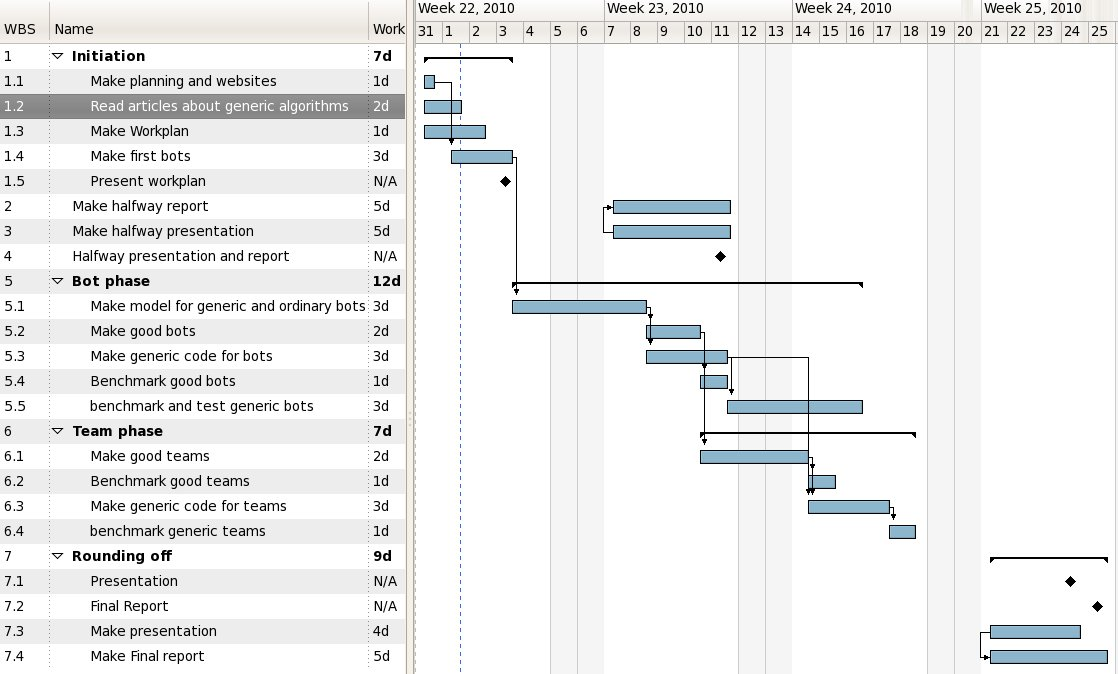
\includegraphics[width=1\textwidth]{Planning_v1.jpg}}
  \end{picture}
%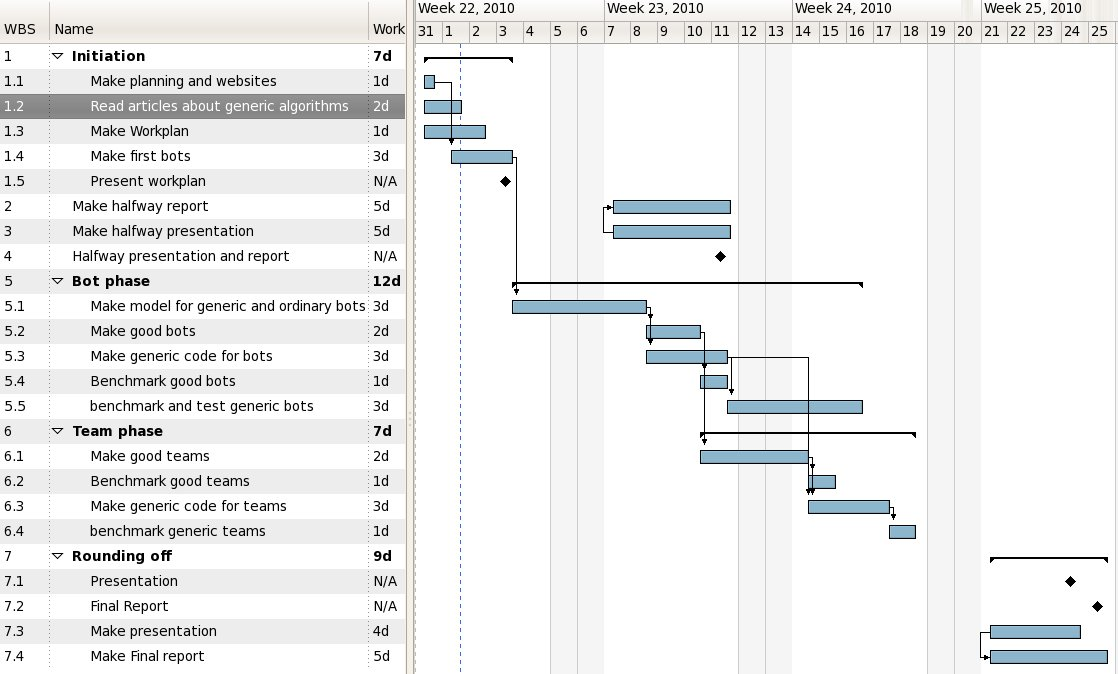
\includegraphics[size=0.0001]{Planning_v1.jpg}
\end{frame}
\begin{frame}
 \thispagestyle{empty}
\end{frame}



\end{document}
